Рассмотрим и произведём вычисление трудоёмкости для классического алгоритма и алгоритма Винограда для умножения матриц $ А[MxN] $ и $ B[NxQ] $

\section{Классический алгоритм умножения}
Данный алгоритм непосредственно использует вышеприведённую формулу. Для вычисления каждого элемента матрицы С 
совершается циклический обход k элементов из таблиц А и B.

Схема алгоритма приведена на рисунке 2.1.
\begin{figure}[h]
	\begin{center}
		{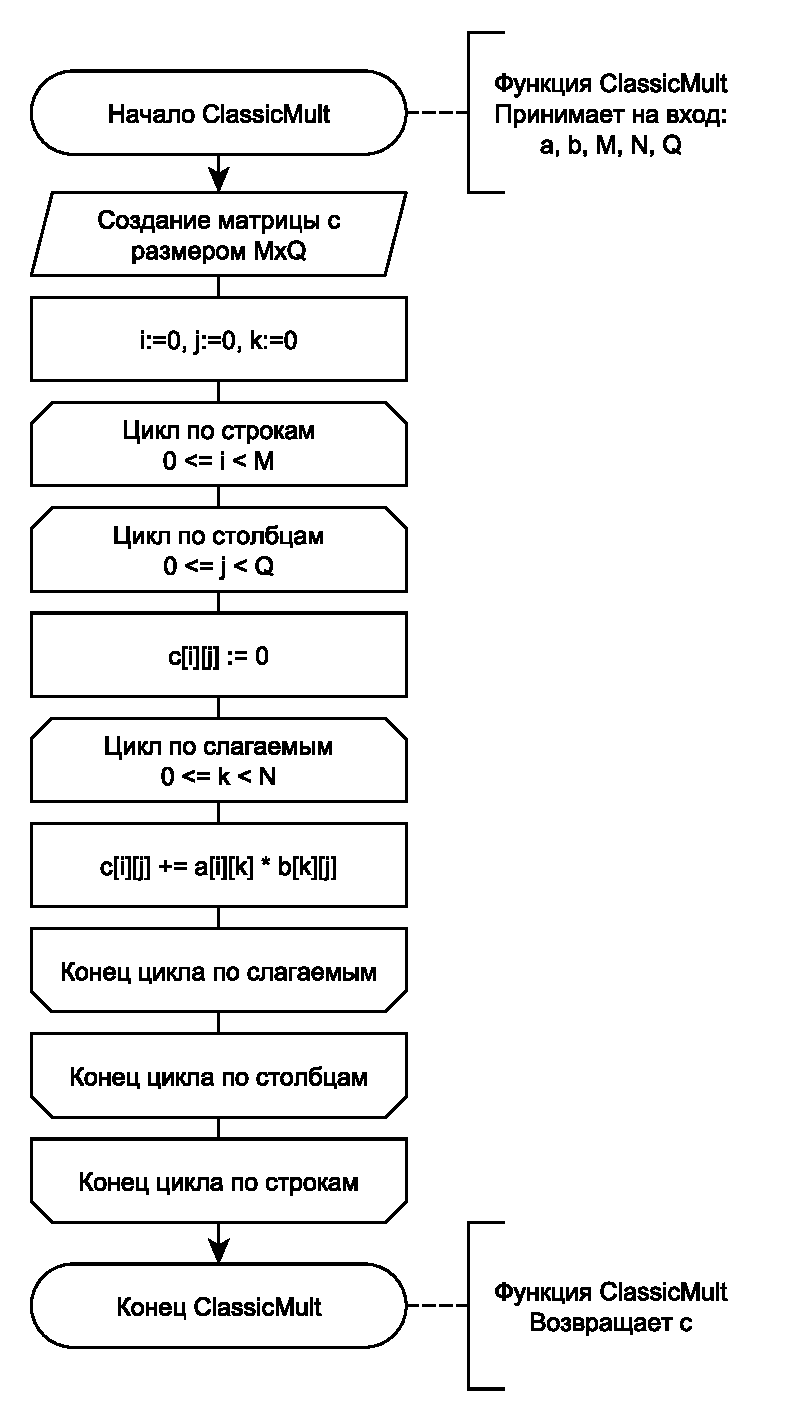
\includegraphics[scale = 0.8]{Classic}}
		\caption{Классический алгоритм умножения матриц}
	\end{center}
\end{figure}

% //////////////
\section{Алгоритм Винограда}
Цель алгоритма заключается в сокращении доли умножений в самом трудоёмком участке кода. Используя вышеописанные соотношения, сначала вычисляются и заносятся в массив вчиатемые для каждого столбца и каждой строки. После происходит вычисление элементов матрицы С. В случае нечётного N дополнительно происходит проход умножения по неучтённым элементам.

Схема алгоритма приведена на рисунках 2.2. и 2.3.
\begin{figure}[h]
	\begin{center}
		{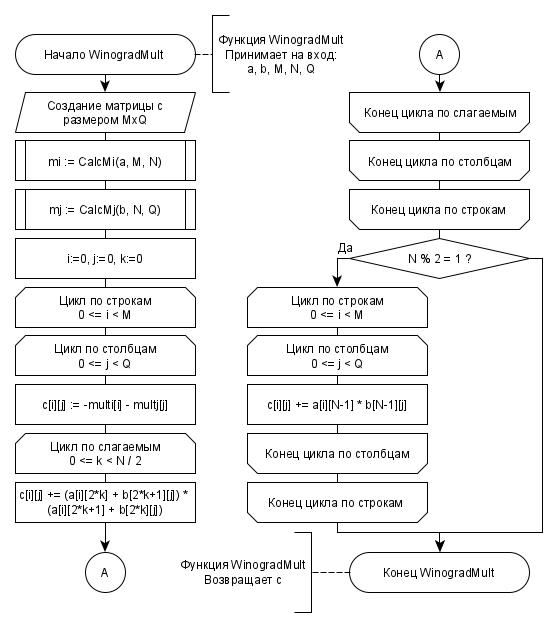
\includegraphics[scale = 0.8]{Winograd1}}
		\caption{Алгоритм Винограда (часть 1)}
	\end{center}
\end{figure}
\begin{figure}[h]
	\begin{center}
		{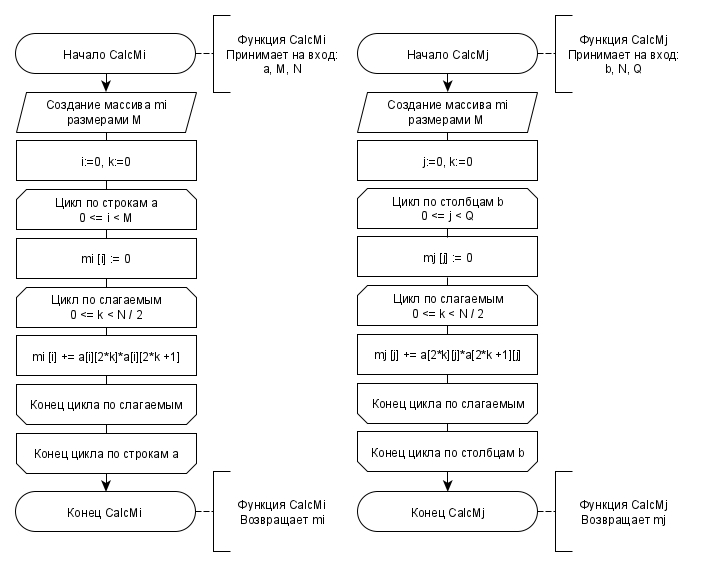
\includegraphics[scale = 0.7]{Winograd2}}
		\caption{Алгоритм Винограда (часть 2)}
	\end{center}
\end{figure}


\section{Оптимизированный алгоритм Винограда}
Для понижения трудоёмкости вышеописанного алгоритма Винограда можно произвести следующие оптимизации:

\begin{itemize}
	\item При вычислении ячеек С, промежеточный результат записывается в временную переменную, которая после получения результата переносится в матрцу С. Таким образом снижено количество операций высчитывания адреса.
	\item Цикл по слагаемым (с переменной k) изменён на аналогичный с шагом 2. Таким образом, внутри цикла не требуется производить умножение k на 2.
	\item Также введена переменная k1, равная k-1. Она, как и k, увеличивается на каждом проходе цикла на 2, и таким образом вместо 2 операций (k-1) за цикл остаётся одна.
	\item Вычисление массива multi заменено на высчитывание значения mi = multi[i] внутри общего цикла. Таким образом удалось избавиться от накладных расходов для цикла и от выделения и освобождения памяти под массив.
\end{itemize}

Схема алгоритма приведена на рисунках 2.4. и 2.5.
\begin{figure}[h]
	\begin{center}
		{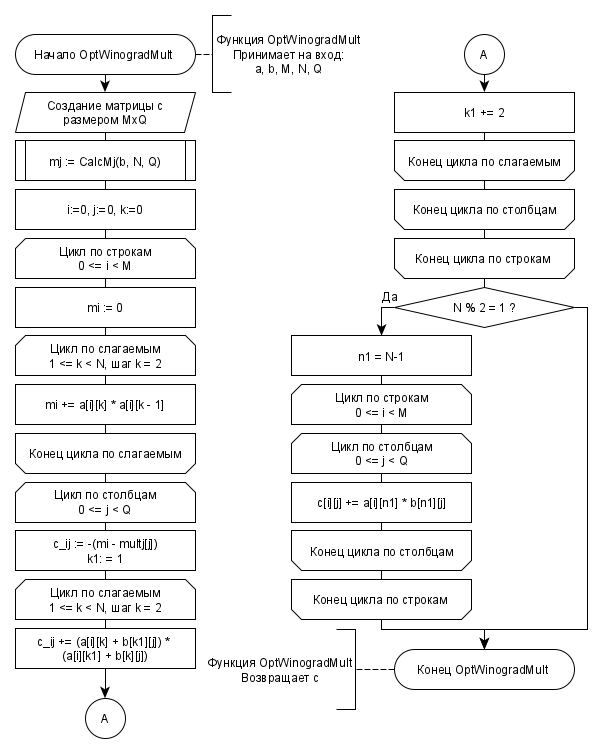
\includegraphics[scale = 0.7]{Winograd_opt1}}
		\caption{Оптимизированный алгоритм Винограда (часть 1)}
	\end{center}
\end{figure}
\begin{figure}[h]
	\begin{center}
		{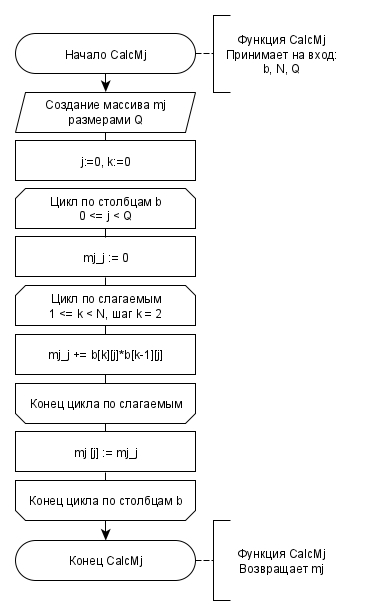
\includegraphics[scale = 0.7]{Winograd_opt2}}
		\caption{Оптимизированный алгоритм Винограда (часть 2)}
	\end{center}
\end{figure}


\section{Требования к программному обеспечению}
Для полноценной проверки и оценки алгоритмов необходимо выполнить следующее.
\begin{enumerate}
	\item Обеспечить возможность консольного ввода двух матриц и выбора алгоритма для умножения. Программа должна вывести результирующую матрцу.
	\item Реализовать функцию замера процессорного времени, затраченного функцией. Для этого также создать возможность ввода размера матрицы, на которых будет выполнен замер.
\end{enumerate}


\section{Заготовки тестов}
При проверке алгоритмов необходимо будет использовать следующие классы тестов:
\begin{itemize}
	\item матрицы размером 1х1, квадратные матрицы;;
	\item две или одна пустая матрица;
	\item чётный и нечётный размер N;
\end{itemize}



